\subsubsection{Localization Daemon}
Because sensor data can be noisy, kinematics models will fail to fully account for wheel slippage, and getting lost is not an option, a particle filter is used in order to refine the pose of the vehicle after every movement.
\paragraph{Initialization}
The initial particle swarm is distributed to match the rules of the competition.  Inside the particle filter, the pose is defined as the sensor position.  In order to cover all possible starting posisitons, the initial particles must be distributed around two circles, one for each potential mining vehicle location.  After chosing a random vehicle location and orientation for a particular particle, the distance between the center of the MMV and sensor is used to determine the particle location.
\begin{figure}[H]
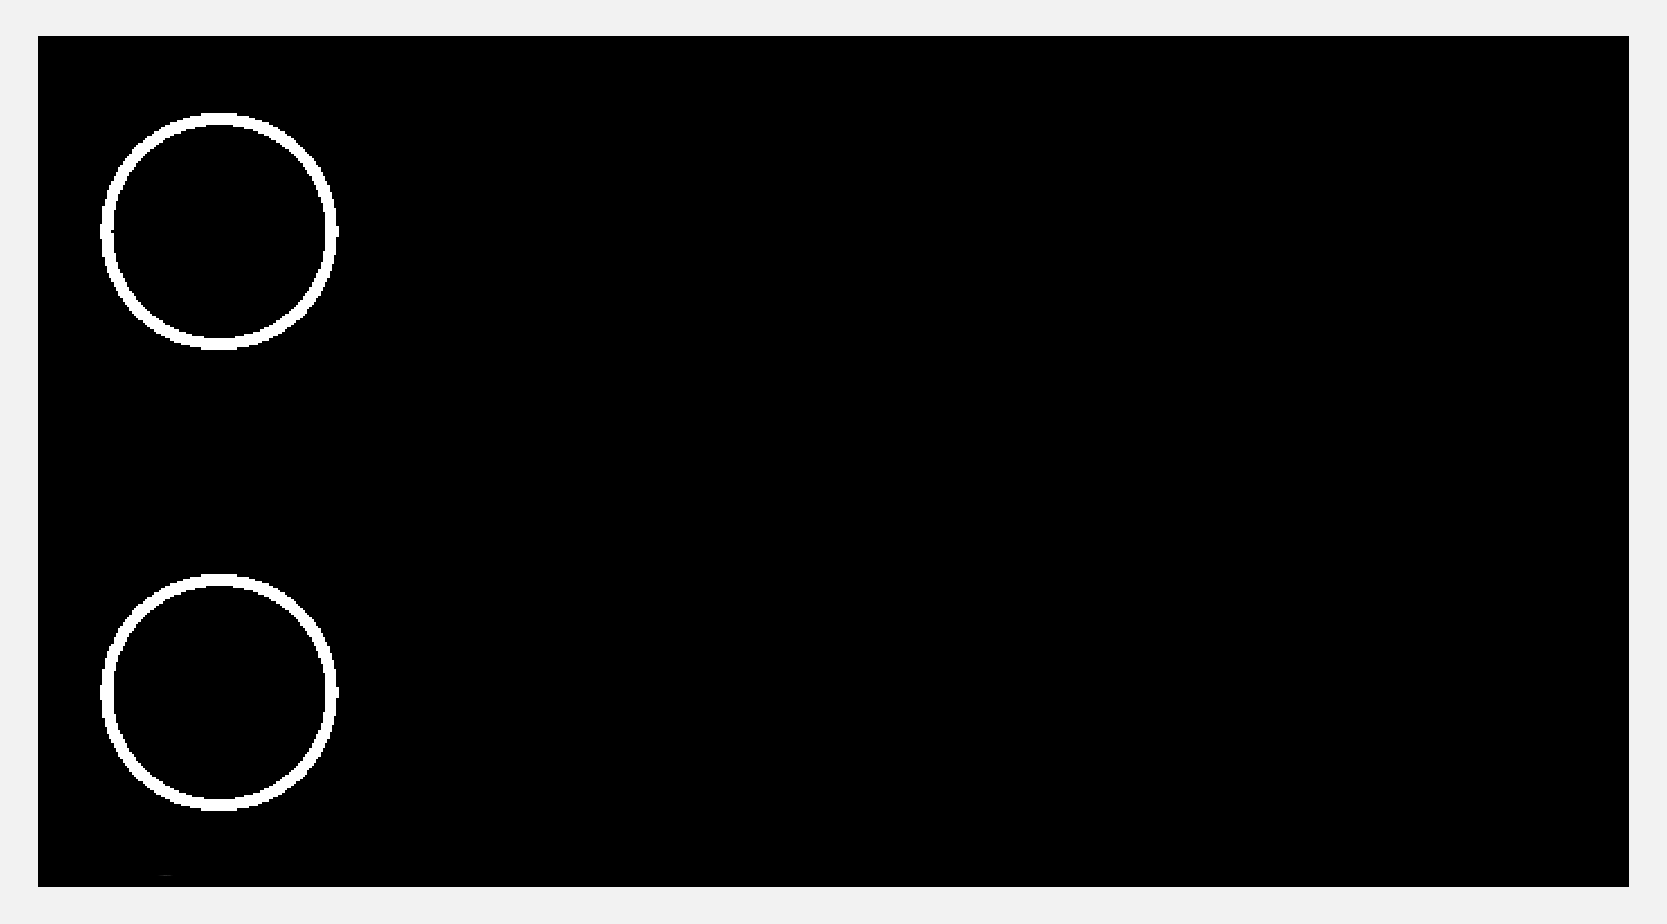
\includegraphics[width=\linewidth]{swarm-init.png}
\caption{Initital swarm distribution}
\end{figure}
\paragraph{Evaluation/Resampling}
The particle filter then proceeds by first evaluating each particle's fitness.  It does this by comparing the LIDAR range data to the known map of the arena, assuming the pose of the given particle.  The fitness of all particles is normalized to create probabilities.  Next, the particles are ordered by probability and resampled.  Those particles with higher probabilities will be chosen more often than those with lower probabilities.  The highest probability particle is saved and returned to the AutonomyHandler as the current pose.
\paragraph{Motion}
After the AutonomyHandler uses the current pose to make a decision and move the vehicle, it first gives the localization daemon a motion vector.  This vector specifies the expected change in $x$, $y$, and $\theta$ for the MMV, as calculated from the kinematics model.  Since this model will likely have accuracy issues due to wheel slippage and imperfect Hall effect sensor data, not all particles have the motion vector applied.  All particles receive a small normally distributed random perturbation for each of $x$, $y$, and $\theta$.  Those particles that did not have the motion vector applied are given a larger perturbation.  In this fashion, the swarm covers all the potential positions of the miner and is once again ready for evaluation and resampling.
